\section{State of The Art}
\label{sec:state_of_the_art}

\subsection{COMPSs}
\label{subsec:compss_state_of_the_art}
\section{The COMPSs Programming Model}
\label{sec:compss}
\subsection{Introduction}
COMP Superscalar (and, from now on, COMPSs) is a framework aimed to ease the development of applications for distributed infrastructures \cite{compss} \cite{Lordan2014}. A COMPSs application is typically a normal application with some special annotations and a few extra function calls in its code that transform a sequential code into a program that can run in a distributed environment.\\
\\
COMPSs applications can be written in Java, C/C++, and in Python (both 2 and 3). The Python framework is called PyCOMPSs \cite{pycompss}. All the examples and real-world usages in this project will be developed in the PyCOMPSs framework and in the Python language. However, this does not mean that all the features discussed and developed in this project are only available for PyCOMPSs. In fact, given how COMPSs is designed, the implementation of a feature for PyCOMPSs usually implies to implicitly implement it for any of the programming languages that are supported by COMPSs.\\
\\
The COMPSs framework also provides users and developers with some tools and data that helps to monitor and to debug the applications and COMPSs itself. From a user point of view, a graph of the workflow and traces of the execution of applications can be generated (figures \ref{fig:graph_example}  and \ref{fig:trace_example}). Traces are generated with a combination of Extrae \footnote{https://tools.bsc.es/doc/pdf/extrae.pdf}, Paraver \cite{paraver}, and a custom implementation inside COMPSs itself. From a developer point of view, many debug information, as logging messages and stack traces, is available if runnning COMPSs with debug flags or in case COMPSs crashes. We must mention that these logs are not always the answer or the solution. For example, if both the master and some worker complain in their respective logs about something some questions should be answered. Some questions, as knowing if some error is the cause or the consequence of some other error that happened elsewhere, are very hard to find and they may take a lot of time to be fixed.  Some of these questions, as knowing which error happened first (assuming they are independent), are even harder to answer \cite{Lamport}. 

\begin{figure}[ht!]
\centering
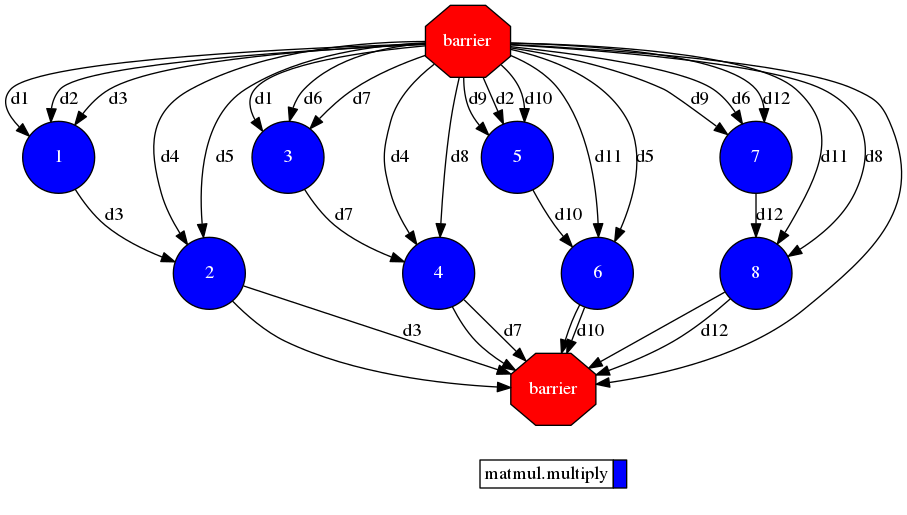
\includegraphics[scale = 0.45]{figures/2x2_matmul_graph.png}
\caption{A dependency graph generated by a COMPSs application. Circular nodes are tasks, octogonal edges are syncpoints, and edges are dependencies between tasks and/or syncpoints caused by some data. The labels of the edges are the identifiers of the data that causes these dependencies.}
\label{fig:graph_example}
\end{figure}

\begin{figure}[ht!]
\centering
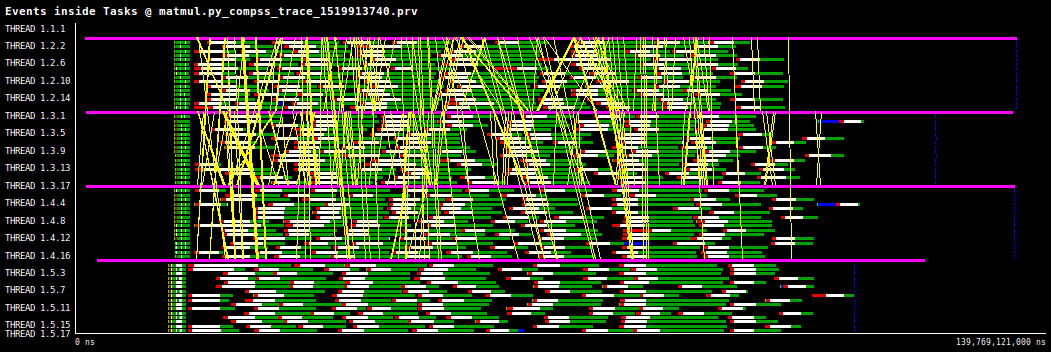
\includegraphics[scale = 0.3]{figures/matmul_trace.png}
\caption{A trace generated by a COMPSs application. Each row corresponds to a process, colored segments are different tasks, and yellow lines are network transfers between different computing nodes.}
\label{fig:trace_example}
\end{figure}

\newpage
\subsubsection{A Full Example}
\label{subsec:compss_example}
This section intends to give the reader a more or less extensive insight on what writing a COMPSs application is. We think that this section may help to \textit{materialize} concepts and will avoid to give this document an excessively abstract tone.\\
\\
Lets suppose that we want to approximate the value of $\pi$. For this purpose we have thought on a simple, randomized algorithm:
\begin{enumerate}
\item Generate $N$ random 2D points with coordinates between $-1$ and $1$
\item Consider the set of points $S$ within distance $1$ or less to the origin
\item Assume that $\frac{|S|}{N} = \frac{\pi}{4}$
\end{enumerate}

\begin{figure}[ht!]
\centering

\includegraphics[scale=0.5]{figures/circle_square.png}
\caption{A graphical representation of the random experiment. The square has side length $2$, so the circle has radius $1$, and therefore area $\pi$. In ratio terms, $\frac{\pi}{4}$ of the points belong to the circle}
\label{fig:circle_square}
\end{figure}

A more graphical explanation on why this works can be found in figure \ref{fig:circle_square}.\\
\\
We know a little bit of Python, so we have decided to implement this program in it. Basically, our small application will consist of a \verb|test_random_point| function that generates a random point and return $1$ if this point lies inside our circle, and $0$ otherwise. We will call this function $N$ times, and consider the proportion $\frac{|S|}{N}$ to be equal to $\frac{\pi}{4}$.
\inputminted{python}{applications/PI_SQUARE/sequential.py}
This code can be straightforward \textit{optimized} by transforming the \verb|test_random_point| function into a COMPSs task and syncing the results in the main procedure.
\inputminted{python}{applications/PI_SQUARE/pycompss_naive.py}
Although this may be a good approach to \textit{parallelize} this application we must note that we want to make it run in a distributed environment. The main difference we can appreciate is that a COMPSs task may run in a different machine than the master code, so some coordination between two processes in different machines and the transfer of potentially big amounts of data are necessary. In other words, the tradeoff between task granularity and performance is much more punishing in distributed computing than in single-machine parallel cases.\\
\\
Another important thing to note is that a distributed application can still exploit lower level parallelism in each of its tasks. In our case, we can transform our \verb|test_random_point| function into a \verb|test_random_points| procedure that generates and tests various random points at the same time.

\inputminted{python}{applications/PI_SQUARE/pycompss_vectorized.py}

This last approach is what we consider a well \textit{COMPSsfied} application: it has a reasonable task count and granularity, and it exploits various levels of parallelism at the same time. This application also delegates most of the work to \verb|numpy| procedures, which are mainly written in C++ and OpenMP. This aspect is also important in PyCOMPSs, as Python is, by nature, a very slow programming language and it should be only used as an orchestrator.

As we mentioned in section \ref{subsec:mare_nostrum}, COMPSs is mainly designed to run in HPC environments. Most of HPC machines integrate some sort of queue system to manage its resources among all the demanding users. Our previous example can be run as a job in a queue system with the following command:

\inputminted{bash}{applications/PI_SQUARE/run_mn4.sh}

The \verb|enqueue_compss| command refers to a generic queueing script (see section \ref{subsec:hpc_queues}) which translates our request to enqueue this COMPSs job to a specific queue system. Some of the most common parameters of a COMPSs job can be found in table \ref{table:compss_queue_param}.\\
\\
\begin{table}[ht!]
\centering
\begin{tabular}{|l|l|}
\hline
Argument name   & Description                                                                           \\ \hline
\verb|exec_time|      & Job time limit                                                                        \\ \hline
\verb|num_nodes|      & \begin{tabular}[c]{@{}l@{}}Number of computing\\ nodes\end{tabular}                   \\ \hline
\verb|cpus_per_node| & \begin{tabular}[c]{@{}l@{}}Number of cores per\\ computing node\end{tabular}          \\ \hline
\verb|constraints|     & \begin{tabular}[c]{@{}l@{}}Additional constraints\\ (e.g: highmem nodes)\end{tabular} \\ \hline
\end{tabular}
\caption{Some example configuration parameters of the queue system. These parameters are usually passed as flags to the enqueue\_compss script.}
\label{table:compss_queue_param}
\end{table}


\subsection{COMPSs Components}
\label{subsec:compss_components}
COMPSs is designed, developed, and deployed in a modular way. This has some advantages:
\begin{itemize} 
\item Easier isolation of features
\item Partial COMPSs installations are possible (e.g: install COMPSs without PyCOMPSs)
\item Components can be individually replaced, leading to faster deployments
\end{itemize}
An overview of the main COMPSs components can be found in figure \ref{fig:compss_modules}. These components are also modularized, as seen in figures \ref{fig:runtime_modules} and \ref{fig:pycompss_modules}.
\begin{figure}
\centering
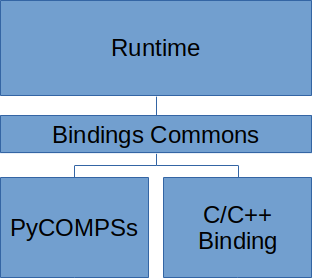
\includegraphics{figures/compss_modules.png}
\caption{Overview of the main COMPSs components.}
\label{fig:compss_modules}
\end{figure}

\begin{figure}
\centering
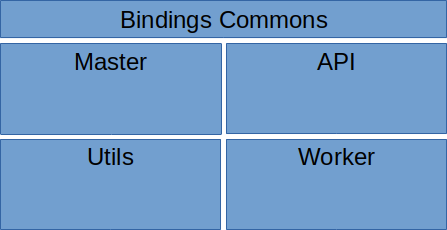
\includegraphics{figures/pycompss_modules.png}
\caption{Overview of the main PyCOMPSs components.}
\label{fig:pycompss_modules}
\end{figure}

This design choice also brings some unwanted problems. The main issue is isolation and concentration of knowledge of some parts in some developers, which leads to unnecessary code replication, lack of coherence of design and implementation choices between different modules, partial feature implementations (e.g: a feature that is only available in PyCOMPSs because it was developed by someone who did not know how to implement it in the Java runtime), and many other things. All these issues will be adressed and referred to in this document, as they appear and play an important role in our own design choices and implementations.

%TODO
\subsection{Runtime Structure}
\label{subsec:runtime_structure}

\begin{figure}
\centering
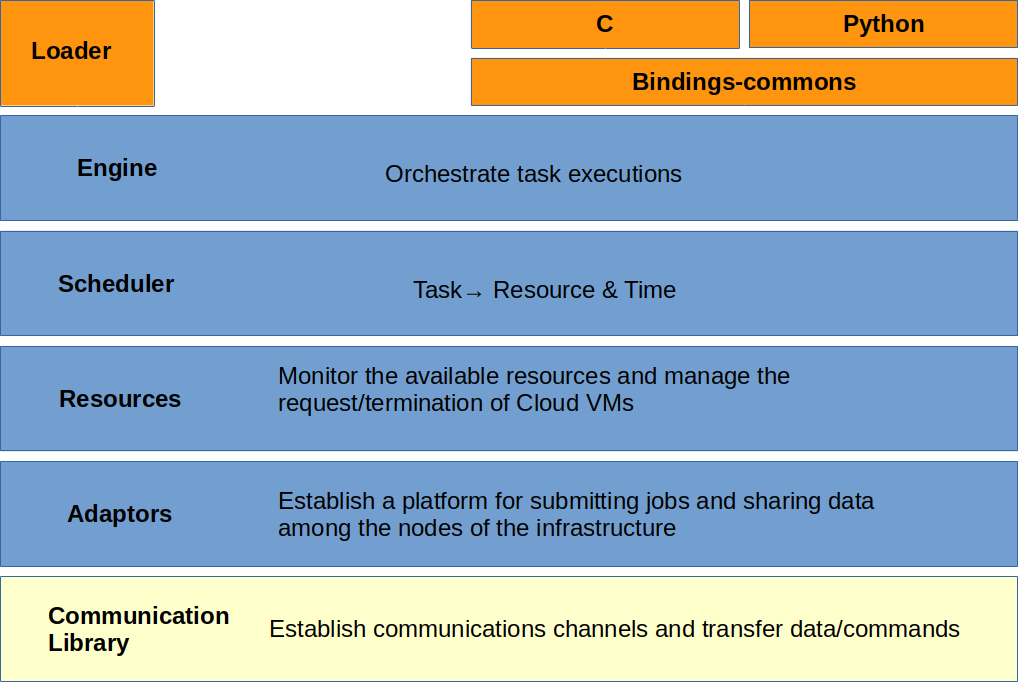
\includegraphics[scale = 0.45]{figures/runtime_modules.png}
\caption{Overview of the main Runtime components.}
\label{fig:runtime_modules}
\end{figure}

\subsection{PyCOMPSs Structure}
\label{subsec:pycompss_structure}
PyCOMPSs can be summarized as a Python Binding for COMPSs. It gives the user a way to annotate his Python code, and it internally transforms and forwards all the derived task creation requests and data to the COMPSs Runtime. Its role can be summarized as follows:
\begin{enumerate}
\item Execute the user code, both the master and the worker part
\item Implement code annotations (\verb|@task|, \verb|@binary|, etc)
\item Implement flow control mechanisms (\verb|compss_wait_on|, \verb|compss_barrier|, etc)
\item Transform the user data into something easily to transport between different machines
\end{enumerate}

\subsection{Usability vs Performance}
\label{subsec:compss_ux_vs_perf}
COMPSs has two goals: to give the not-so-expert user an easy way to make their sequential applications run in distributed environments, and to do it as efficiently as possible. Many improvements in the COMPSs framework are aimed to improve only one of these two aspects. For example, any improvement in the communication library may improve the performance of the user application, but the user will still face the same usability limitations when using COMPSs. Adding an automatic return completion, to handle the case when the user forgot to annotate the return value of some task, may save the user a lot of debugging time, but it will have no impact in the performance of the user application.\\
\\
The COMPSs software is developed and mantained by a research team in a research center, so it may be natural to think that most of the efforts and improvements are aimed to test and develop methods, models, and algorithms that improve performance, memory usage, minimize network transfers and so on. However, COMPSs is also used by other research teams as a \textit{tool} for their own purposes. Some of these teams intend to run exotic, old, complicated applications in distributed environments. Also, these teams are usually composed of researchers from different fields than computer science, so a lack of knowledge in parallel and distributed applications should be expected. The user-oriented features intend to help these research teams, and to make their life easier in the very complicated world of distributed computing. These two big forces (being a research team and having \textit{clients}) act as the main source of ideas and features in the COMPSs environments, and they are not always acting towards the same direction.\\
\\
This project tries to bring something that improves COMPSs in these two directions: give something to the user that makes his life easier while making COMPSs more efficient. For example, we do not intend to limit ourselves to give the user a way to pack some parameters in a collection. We see this feature as an opportunity to give COMPSs additional intelligence that may help to improve the performance of the framework. The same applies with the storage interface. Our goal is twofold: to give the user a way to make his or her COMPSs application run with other storage systems and to take advantage of these systems in terms of performance.


\subsection{Mare Nostrum IV}
\label{subsec:mare_nostrum}
%TODO: MENCIONAR QUE COMPSS ESTA PENSADO PARA SER USADO AQUI
Mare Nostrum is a generic name to refer to the main supercomputer of the Barcelona Supercomputing Center \footnote{https://www.bsc.es}. Mare Nostrum IV is the fourth version of this supercomputer.

\subsection{GPFS}
\label{subsec:gpfs}
GPFS \cite{schmuck2002gpfs} is a distributed file system developed by IBM. It gives a perceived behaviour of a regular POSIX file system, while guaranteeing consistency between different computational resources, and a correct parallel access to its files. Under this model, any node has access any file at any location. As we can see in figure \ref{fig:gpfs_schema} a node accesses data through a switching fabric. A switching fabric is a kind network topology in which any two nodes connect between each other through a series of switches. This topology allows a more efficient communication between nodes than other topologies such as broadcast networks.
\begin{figure}
\centering
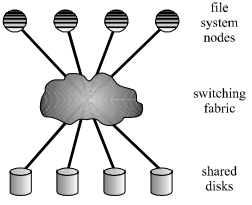
\includegraphics{figures/gpfs_schema.png}
\caption{GPFS Shared disk environment. Figure 1 from \cite{schmuck2002gpfs}}
\label{fig:gpfs_schema}
\end{figure}
GPFS is available at the Mare Nostrum IV supercomputer, and COMPSs takes advantage of it by delegating the file system many tasks such as file transfers, consistency across computational resources, and so on. It also makes task scheduling easier, as the data locality factor can be ignored by the COMPSs scheduler, focusing only on load balancing. Being more specific, if COMPSs runs under a GPFS file system it will consider that any piece of data is available anywhere, instead of explicitly keeping track of its locations.

\subsection{Queue Systems - SLURM and LSF}
\label{subsec:hpc_queues}
Most supercomputers have many concurrent users. All of these users want to use some of the resources of the supercomputer, and usually in a selfish manner. This situation creates a lot of conflicts between users, and even some unethical behaviors such as some user killing the processes of other users. Also, many benchmarks and experiments require no noise introduced by concurrent, unrelated processes running in the same machine, so resource exclusivity must be guaranteed in these cases.\\
\\
The most common solution to the two aforementioned problems is to divide the different nodes of a supercomputer into login nodes and computing nodes. When a user opens a session in some supercomputer he will \textit{land} into some login node. Computing nodes are unreachable or even not visible by regular users, and the only way to have access to them is to ask the system for resources and wait until the system lends them to the user. The most common implementation of this resource assignment mechanism is a queue system. A queue system processes all the requests from the users, gives them a priority as a function of various parameters and lends them the requested resources according to these priorities, as a process scheduler does with processes in an operative system.\\
\\
Two of the most common queue systems are LSF \cite{zhou1992lsf} and SLURM \cite{yoo2003slurm}. All the experiments of this project will be done in the Mare Nostrum 4 supercomputer, which uses SLURM.\\
\\
Although SLURM has its own micro-language and instructions, such as \verb|srun|, and submissions scripts, most of the experiments done in this project will not need them, as we will have generic queueing scripts available to us. A generic queueing script is a script capable to work with various queue systems to generate the corresponding specific queueing scripts. In our case, our script will translate our orders into a bunch of \verb|srun| commands and similar.\\
